%----------------------------------------------------------------------------
\chapter{Szakirodalmi áttekintés}
\label{sec:Szakirodalom}
%----------------------------------------------------------------------------
\section{Szenzorok megoldásai}
%----------------------------------------------------------------------------
\label{szenzorok_szakirodalom}

A szenzorválasztás a tervezési folyamat egyik központi eleme. Meghatározza milyen technológiákkal, módszerekkel hajtjuk végre a méréseket, és ezáltal milyen kapacitású, programozású rendszert kell válasszunk. A szenzorokat érintő kutatómunka ezt a választási folyamatot segíti elő, hiszen az összes népszerű lehetőség tudatában lehet egy informált döntést hozni. Itt tárgyalva lesznek a különböző mérési elvek, amelyek a mért test követelményeit is meghatározzák. Ezen felül bizonyos esetekben a mérési elv által megengedett szenzorkialakítások is bemutatásra kerülnek.

\subsection{Mérendő mennyiségek}

A feladatom során, a nyomatékhatároló csúszásának meghatározásához az azt megelőző és azutáni tengelyek fordulatszámának összehasonlítására van szükség. A harmadik fordulatszámmérés a felszedő tengelyen történik meg, kifejezetten az operátor informálása céljából. Egy tengely fordulatszámának mérésére több megközelítés is létezik. Lehetséges a tengely elfordulásának közvetlen mérése, akár fordulatonként egyszer történő jeladás regisztrálása, vagy a tengely kerületén érzékelhető folyamatos változás. A fordulatszám más mért mennyiségekből is származtatható, például integrálás útján gyorsulásmérésből, vagy deriválással szögelfordulásból, azonban ezeknek a pontossága nem minden esetben megfelelő, valamint a számítási igénye is magasabb az ilyen módon származtatott jeleknek \cite{Morris2016a}.

\subsection{Elmozdulás mérés}
\label{elmozd}

Az elmozdulás egy tengely mentén való mozgást jelent. Ennek mérése általában egy adott tartományon belül alkalmazható, így folyamatos elmozdulás mérésére a szenzorok nagy része nem alkalmas. A fordulatszám mérés esetén az elmozdulás szenzorok felhasználása általában a kerület mentén történő távolságbeli különbség érzékelésére valósul meg. Erre a kerület menti geometriát (pl. fogaskerekek), egy segédlemezzel kialakított változást, vagy akár egy felhelyezett jeladó (pl. mágnes) érzékelés is mérhető.

\subsubsection{Potenciométer}
\label{linpot}

Az elmozdulás vagy pozíció érzékelésének alapvető szenzora a potenciométer, amely akár lineáris, akár elfordulás mérésére is alkalmas. 
A potenciométer működési mechanizmusa a vezetékek ellenállásán alapszik. Egy vezeték ellenállása lineárisan növekszik a hosszával, így a hosszának változása a rajta eső feszültségen keresztül mérhető. A hosszváltozás eléréséhez egy csúszka teremt kapcsolatot a vezetékkel, amelyen a vezeték végéhez képesti potenciált mérjük. A potenciál a \ref{poti} összefüggésből kapható meg, ahol $E$ a tápfeszültség, $d$ az elmozdulás, $D$ pedig a teljes elmozdulás \cite{Fraden2016a}.
\begin{equation}
	V = E \frac{d}{D}
	\label{poti}
\end{equation}
A potenciométeres szenzoroknak többféle megvalósítása is létezik. A legalapvetőbb lineáris vezeték elvén egy tekercset is lehetséges vezetékként használni, így valamivel pontosabb, nagyobb felbontású érzékelést eredményez. Léteznek potenciálmérés alapú nyomásmérő, valamint piezoelektromosságon alapuló deformáció mérésre alkalmas cellák \cite{Fraden2016a}.
Az elektromos potenciál alapú szenzorok széles felhasználásuk mellett rendelkeznek számos hátránnyal is:
\begin{itemize}
	\item Mechanikai terhelés által súrlódás
	\item Fizikai érintkezés szüksége
	\item Korlátozott sebesség
	\item Veszteségek miatti hő termelődés
	\item Szennyeződések és kopásoknak való kitettség
\end{itemize}
A fizikai kontaktus elkerülésére alkalmaznak mágneses elven működő potenciométereket. Ezeknél a szenzoroknál a csúszka egy ferromágneses bevonattal van ellátva, a vezeték alatt pedig egy mágneses réteg helyezkedik el, amelyet a csúszka vonzása összeérint a vezetékkel, így zárva az áramkört és feszültséget adva az eszközre.

\subsubsection{Kapacitív szenzorok}

A kapacitív érzékelők elmozdulás és pozíció meghatározására is alkalmasak, a későbbiekben ismertetésre kerülő mágneses alapú szenzorokkal ellentétben, bármilyen anyag jelenlétét képesek érzékelni.A kondenzátorok (kapacitív áramköri elemek) kapacitása fordítottan arányos a fegyverzetek közötti távolsággal, ami meglapozza a kapacitív szenzorok működését. A kapacitás változását a távolság változása vagy a fegyverzetek között található közeg változása okozhatja, amely a gyakorlatban elmozdulásmérésre alkalmas, a kapacitás változásának elektromos jellé alakításával.

 A \textit{monopoláris} kapacitív érzékelő, egy kondenzátor, vagyis két fegyverzet alkalmazását jelenti. Az egyik fegyverzeten mérhető az elektromos jel, a másik fegyverzet azonban lehet például egy vezető felület is, mint ahogy a \ref{kapacitiv_kabel} ábrán látható szenzor kialakítása is mutatja. Ezek a szenzorok akár 40 kHz-es mérési frekvenciát is képesek produkálni, illetve alacsonyabb pontossággal akár nem vezető felületeket mérésére is alkalmasak.
\begin{figure}
	\centering
	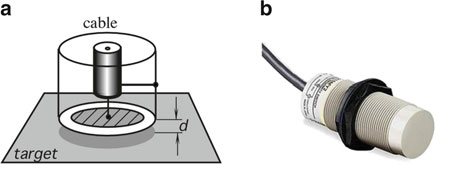
\includegraphics{figures/kapacitiv_szenzor_kabeles.png}
	\caption{Monopoláris, egylemezes kondenzátor vezető felületek távolság mérésére alkalmazva. (\textbf{a}) metszetként; (\textbf{b}) kívülről \cite{Fraden2016a}.}
	\label{kapacitiv_kabel}
\end{figure}
Egy másik kialakítás a differenciál kapacitív érzékelő, amely során három fegyverzet két egyforma térrészt választ el. A középen elhelyezkedő lemez legkisebb mozgása során is megjelenik az így kialakult két kondenzátor kapacitásán, és egy változó jellel táplálva a pontos elmozdulás meghatározására is képes.
Egy kapacitív hidat látunk a \ref{kapacitiv_hid} ábrán. A szenzor két párhuzamosan elrendezett elektróda készletből állnak, konstans $d$ távolsággal közöttük, melyek közül a négy lemezből álló készlet statikus, míg a két fegyverzet elmozdulhat. A négy lemez keresztbe van kötve, így kialakítva az úgynevezett Wheatstone-híd architektúrát, melynek előnye, hogy a mérés linearitását megtartja, valamint a zajok megjelenését is minimalizálja. A párhuzamos lemezek kapacitása arányos a vele szemben lévő fegyverzetek területével, így a két kondenzátor egymáshoz képesti kisebb elmozdulását vagy elfordulását is képes detektálni. 
\begin{figure}
	\centering
	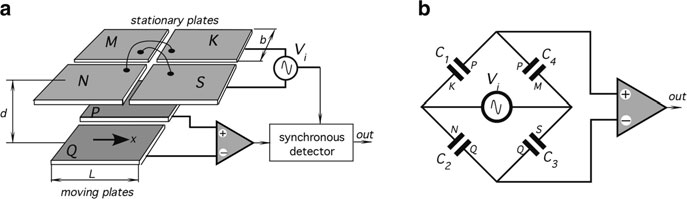
\includegraphics{figures/kapacitiv_hid.png}
	\caption{Párhuzamos lemezű kapacitív híd szenzorbeli elhelyezése (\textbf{a}) és áramköri rajz (\textbf{b}) \cite{Fraden2016a}.}
	\label{kapacitiv_hid}
\end{figure}

\subsubsection{Induktív szenzorok}
\label{linind}

Induktív szenzorok azok, amelyek mágneses terek tulajdonságait érzékelik, és így csak olyan anyagok detektálására alkalmasak, amelyek kölcsönhatásba lépnek a mágneses mezővel. A rozsdamentes acél, alumínium, réz, műanyag, kerámia és fa anyagok áthatolhatóak a mágneses terek szempontjából, így ezekből az anyagokból készült rétegeken keresztül is érzékelhetőek a mágnesezett anyagok. Az induktív szenzorok ezáltal működnek zajos, szennyező (poros, olajos) környezetben is, valamint ezáltal az érzékelőkön a helyzetnek megfelelő anyagból készült burkolatokat lehet alkalmazni, amely veszélyesebb, korrozívabb helyzetekben is megengedi működésüket.\\
Több elv alapján és több kialakítással is érzékelhetjük a mágneses tereket.
\begin{itemize}
	\item \textbf{Elektromágneses indukció}. Két tekercs között mágneses fluxus biztosít kapcsolatot, amelyhez kell az első (primer) tekercs változó áramú gerjesztése, mely így - fázisban - megjelenik a második (szekunder) tekercsen is (önindukció elve). Ezt a kapcsolatot tudják befolyásolni különböző ferromágneses anyagok, a fluxus utakban való mozgatásuk során, ezáltal a fluxus módosításával. Ez a fluxusbeli változás mérhető feszültség változást eredményez a szekunder tekercsen. Ez adja a lineáris (és a forgó) változó differenciális transzformátor (LVDT - Linear Variable Differential Transformer) szenzorok alapjait, amelyek ferromágneses anyagok lineáris- vagy forgómozgását képesek érzékelni a két tekercs közötti mágneses térben. Ennek a kialakításnak számos előnye van, például az érintkezésmentes kialakítás, elhanyagolható hiszterézis, így kevés feszültségveszteség a működés során, alacsony kitettség zajoknak és interferenciáknak, robusztus kialakítás és infinitezimális felbontás lehetősége \cite{Fraden2016a}.
	\item \textbf{Örvényáramok}. Az örvényáramok két esetben jelennek meg: amikor egy vezető elmozdul egy elektromágneses térhez képest, vagy a mágneses tér változása következtében. Az örvénylő elektronok a vezető anyagban saját elektromágneses mezőket indukálnak, amelyek az eredeti mágneses teret csökkentik. Ha erősebb a mágneses tér, vagy nagyobb a vezetőképessége az anyagnak, vagy gyorsabban változik a mágneses tér, akkor arányosan több örvényáram jön létre. Ezáltal olyan vezető anyagok elmozdulását is lehet érzékelni, amelyek nem mágnesezhetők. Az ezen elven alapuló szenzorok két tekercset alkalmaznak, az egyik referenciaként szolgál, a másik pedig érzékeli a vezetőben létrejövő örvényáramokat, a mágneses ellenállás megnövekedéséből. A két tekercs összehasonlítása során a mágneses ellenállás különbségből adódik a vezető felület távolsága. Az örvényáramok azonban egy adott vastagságú anyagban számottevőek, így a vékony filmszerű illetve bevonattal ellátott anyagok detektálására nem alkalmasak az ilyen szenzorok. Hasonló elven az örvényáramszenzorok nem csak elmozdulás, de távolság és anyagvastagság meghatározására is alkalmasak. Az érzékelő tekercsek akár 2-3~mm-es átmérőtől 25~mm-ig terjedhetnek, így nagy mérési tartomány lefedésére képesek. A nem mágneses vezetők érzékelése miatt alkalmas olyan magas hőmérsékleten való érzékelésre, ahol az anyagok elvesztik mágneses tulajdonságukat (Curie hőmérséklet felett), valamint vezető folyadékok, így folyékony fémek is érzékelhetőek az örvényáramszenzorokkal. További előnyei, hogy nincs fizikai kapcsolatra igény az detektáláshoz, így a terhelés mindig alacsony a szenzoron \cite{Fraden2016a}.
	\item \textbf{Hall-effektus}. A Hall-effektus szenzorok lényegében a mágneses terek nagyságát képesek mérni. A szenzorban egy vezető anyagból készült lemez merőlegesen áll a mágneses térre, ahogy azt a \ref{hall_effektus} ábra is szemlélteti. Ha a vezetőben áram folyik, az elektronokra a mágneses mező oldalirány erőt fejt ki (Lorentz-erő), ezáltal a lemezben töltésmegoszlás jön létre, amely a két szélén Hall-feszültségként mérhető \cite{Fraden2016}. A Hall érzékelős pozíciómérés során egy mágneses mezőt biztosítunk a szenzorban, amelynek a nagysága változik egy ferromágneses test jelenlétében. A szenzortól való távolság pedig, az így indukált mágneses tér módosulásából eredő feszültség változásból következik \cite{Morris2016}. 
	\begin{figure}
		\centering
		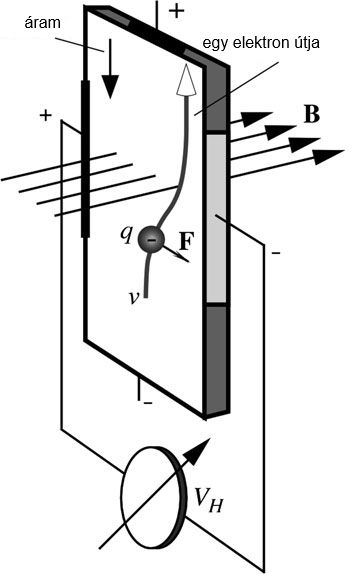
\includegraphics[width=\columnwidth/4]{figures/hall_effektus.png}
		\caption{Hall-effektus szenzor működési elve \cite{Morris2016}.}
		\label{hall_effektus}
	\end{figure}
	\item \textbf{Induktoszin} A lineáris induktoszin (angol: linear inductosyn) egy precíziós eszköz, amelyet szerszámgépek irányításánál alkalmaznak, a $2,5$~\textmu m pontossága miatt. A szenzor két mágnesesen kapcsolt, levegővel elválasztott alkatrészből áll, egy sínből és egy csúszkából, melyeknek elrendezését az \ref{indszin} ábrán láthatjuk. A sín a mérés tengelyének mentén van elhelyezve, a csúszka pedig a mozgó eszközön, szerszámon. A sín felületén -- amely több méter is lehet --, üveg alapba egy fém szál van elhelyezve négyzethullám alakban, amely szinuszos feszültséggel van gerjesztve. A csúszkában található tekercsekben feszültség indukálódik, amely egy négyzethullámon belül pozicionálja a csúszkát (nagyjából 2 mm). Mivel ez az egy hullámhossznyi mérési tartomány igen csekély, a lineáris induktoszin általában egy másodlagos kevésbé pontos távolságmérővel van párosítva \cite{Morris2016a}.
	\begin{figure}
		\centering
		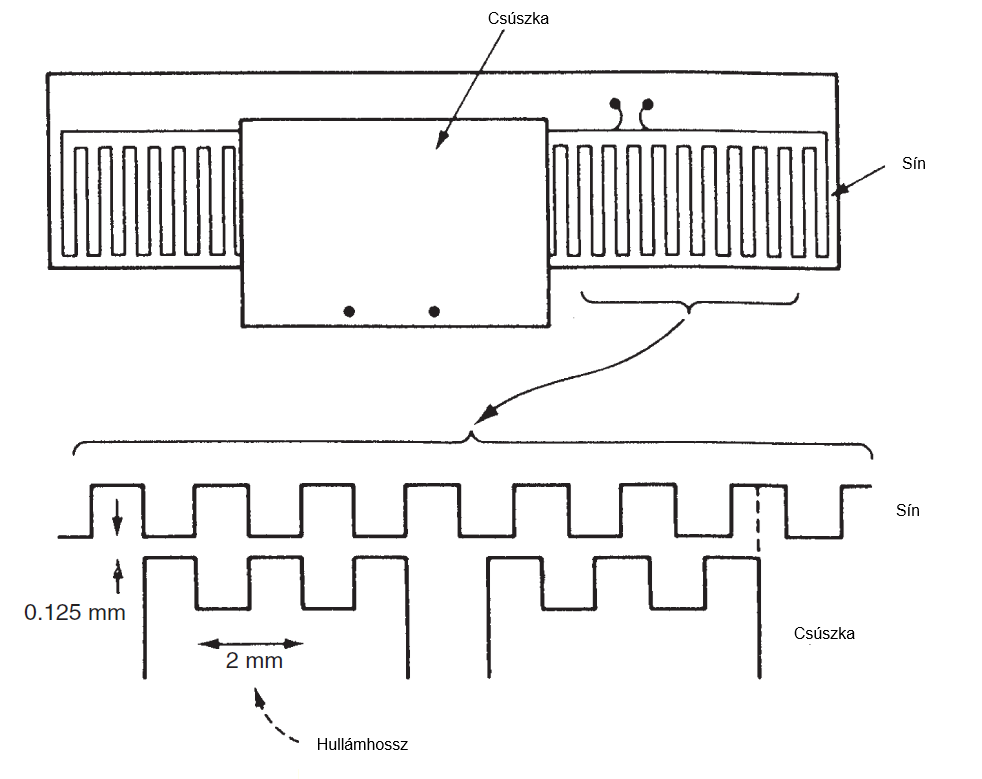
\includegraphics[width=\columnwidth*8/10]{figures/indszin.png}
		\caption{Lineáris induktoszin sematikus rajza \cite{Morris2016a}.}
		\label{indszin}
	\end{figure}
\end{itemize}
Összességében a mágneses szenzorok előnye, hogy nagy felbontással és megbízhatósággal dolgoznak, valamint nincs szükségük mechanikai kapcsolatra a mérés véghezviteléhez. Azonban nagyrészt csak mágneses anyagok detektálására képesek (némelyik vezetőkön is működik), és a mérési távolságuk általában limitált.

\subsubsection{Optikai szenzorok}

A pozíció és elmozdulás mérésére alkalmas optikai szenzorok általában legalább 3 komponensből állnak: egy fényforrás, fényérzékelő és a fényt irányító eszközök, mint a lencsék, tükrök és optikai szálak. Az optikai érzékelők előnyei az egyszerűségük, a relatív nagy mérési tartományuk, valamint a terhelés és érintésmentes mérés. Ezen felül a mágneses és elektrosztatikus zajok nem befolyásolják működésüket, így az erre érzékeny környezetekben is remekül alkalmazhatóak \cite{Fraden2016a}.\\
Az optikai szenzorok különböző kialakításuk szerint néhány fő kategóriába sorolhatók.
\begin{itemize}
	\item \textit{Optikai híd}. A korábban említett Wheatstone-híd elrendezés alkalmazható akár a fotodetektorokra is. Egy detektor minden negyedében egy fényérzékelő, a híd elrendezésnek megfelelően bekötve, ezáltal a negyedek közötti fényerősség különbség jelenik meg feszültségkülönbségként. A jel felhasználása pozíció meghatározásához egy olyan optikai rendszer kialakítása szükséges, ahol az elmozdulás következtében a megjelenő fénysugarakat a negyedek egyikére irányítják.
	\item \textit{Polarizáció}. A polarizált fényről akkor lehet beszélni, ha a fotonok azonos irányba álló mágneses és elektromos terekkel rendelkeznek, amelyet egy polarizáló szűrővel lehet létrehozni. Ha visszaverődik egy polarizált fény, általában a fémes felületekről azonos irányban teszi, nem fémes anyagoknál pedig megváltozhat a polarizáció iránya. Így bizonyos anyagok kizárását vagy mérését lehetővé teszi a polarizációs filterek alkalmazása a fényforrás után (kimenet) és a detektor előtt (bemenet).
	\item \textit{Fabry-Pérot interferométer}. Ennek a szenzornak a működéséhez egy Fabry-Pérot optikai üregre van szükség. Az üreg két szemközti oldalát tükrök borítják egymástól $L$ távolságra. Az üregbe bevilágítva egy ismert fényforrással, a fotonok visszaverődnek mindkét tükör felületéről, így eltárolva a fényt. Bizonyos frekvenciák azonban ki tudnak jutni az üregből, amit a két tükör távolsága határoz meg \cite{Fraden2016a}. A kitörő fény frekvenciájának mérésével lehetséges meghatározni a két tükör távolságát, így nagy felbontású elmozdulásmérést végezve, mely főleg nyomás és hőmérséklet változás detektálására alkalmas.
	\item \textit{Rácsérzékelő}. A fényforrások intenzitásának beállítását el lehet végezni két rács átfedésének állításával. Az egyik rács a jel $50\%$-át kitakarja, ezzel tökéletes átfedésben a második szűrő nem módosít ezen, azonban az elmozdulásával fordítottan arányos a maradék intenzitás. Az elmozdulás nagy tartományon is mérhető ismétlődő intenzitásváltozásokkal, azonban nagy haszna van tárcsák forgómozgásának mérésénél, amely a \ref{optarcsa} fejezetben lesz tárgyalva \cite{Fraden2016a}.
	\item \textit{Lineáris optikai szenzor}. Az infravörös tartomány közeli frekvenciákkal való mérés akár rövid vagy hosszú távú optikai mérésre is alkalmazható. Az infravörös LED (fény kibocsátó dióda) ismert szélességű impulzust bocsájt ki, így az intenzitása ismert. A kibocsátott fényre merőlegesen, a LED-től adott távolságra elhelyezkedő detektor a fény intenzitás felhasználásával egy áramerősség kimenettel biztosítja a távolság háromszögelésének lehetőségét \cite{Fraden2016a}. Az infravörös fény népszerű alkalmazása kis távolságoknál közelségérzékelőkben jellemző. Egy bizonyos távolságon belül a detektorba érkező visszavert fény intenzitása átlépi a határértéket, így a fototranzisztor vezető állapotba kerül és jelet ad \cite{Morris2016c}.
\end{itemize}
Az optikai szenzorok hátránya, hogy fizikai szennyeződésekre, és a fényt továbbító közeg sűrűségére érzékenyek lehetnek. Ennek kiküszöbölésére alkalmazhatóak az optikai szálak, amelyek a detektor és a fényforrás között egy tökéletes visszaverő környezetet biztosítanak, azonban ezek használata limitálhatja az optikai szenzorok alapvetően széleskörű alkalmazási lehetőségeit.

\subsubsection{Ultrahang szenzorok}

Az ultrahangos energiával rendelkező szenzorok a távolság- és sebességmérésben is nagy népszerűségnek örvendenek, a egyszerű kialakításuk és költséghatékonyságuk miatt. Az ultrahang szenzorok az emberi hallás felett, 20 kHz körüli mechanikai akusztikus hullámok kibocsájtásán és érzékelésén keresztül működnek. Ezek felhasználása során lehetséges transzmissziós vagy visszaverődéses rendszerek kialakítása is. Visszaverődő hullámok a sebességmérés területén használatosak, mivel a mozgó tárgyak a visszaverődő jelek hullámhosszát módosítják -- távolodva hosszabbítják, közeledve pedig rövidítik (Doppler effektus) -- \cite{Fraden2016a}. Mivel ezek a jelek terjedési sebességei jóval alacsonyabbak mint a korábban említett elektromágneses sugarak, a mérésük is egyszerűbben és költségtakarékosabban megoldható. Az \ref{uh_eq} egyenletben látható a távolságmérés számítása, az említett $t$ idő, a hullám adott közegbeli terjedési sebessége, valamint a $\Theta$ visszaverődési szög függvényében. Amennyiben a $\Theta$ jeladó és -vevő közötti visszaverődési szög elhanyagolhatóan kicsi (tart a $0$-hoz), az egyenletben szereplő $\cos{\Theta} \approx 1$ lesz, így a távolság valójában csak a sebesség és idő függvényeként jelenik meg.
\begin{equation}
	L_0 = \frac{v t \cos{\Theta}}{2}
	\label{uh_eq}
\end{equation}
A mechanikai hullámok képesek a gáz, folyadék vagy szilárd halmazállapotú közvetítő közegekben is terjedni, azonban a terjedési sebességük a közeg sűrűségétől függ, amely különböző közegek detektálására ad alapot (például víz magasságának mérése). Az elektromágneses hullámokkal ellentétben, fizikai mozgás során lehetséges mechanikai hullámokat generálni. Az ultrahang esetében ez piezoelektromos kerámiákkal valósítható meg, amelyek elektromos gerjesztés hatására méretüket változtatják. A piezoelektromos hatás visszafelé is működik, így a fizikai erőhatás mozgására elektromos jeleket generálnak a kerámiák, amelyek így az érzékelési feladatot is képesek ellátni \cite{Fraden2016a}. Az ultrahangos szenzor előnye, hogy megfizethető, egyszerű kialakítású, nincs szüksége fizikai kapcsolatra és a legkülönbözőbb anyagokon keresztül is alkalmazható. Azonban a mérési frekvenciája korlátozott a jel oda-vissza terjedésére, valamint a közeg tulajdonságai -- hőmérséklete, páratartalma -- merőben befolyásolják a mérés menetét.

\subsubsection{Radarok}

A radar technológiák közül a kis távolságok mérésére a mikrohullám-impulzus radar alkalmazható. Ez a technológia fehér zaj emittálását végzi rövid impulzusokban. Mindegyik kibocsátott zaj adott ideig tart, azonban a kibocsátás ideje véletlenszerű. Ezeket a magas frekvenciás rádióhullámokat egy antenna továbbítja a levegőben, majd érzékeli a visszaérkező impulzusokat. A tárgyakról visszaverődő zaj csomagok között eltelt időt felismeri az azt kibocsátott szenzor, így a kibocsátás és érzékelés között eltelt időből lehet a távolságot számolni. Mivel számítható, hogy milyen intervallumban kell visszaérkezzenek a rádióhullám-impulzusok, a mikrohullám-impulzus radar alacsony energiafogyasztással operál. További előnye, hogy a kibocsájtott fehér zaj detektálása és megzavarása közel lehetetlen. A véletlenszerű impulzus eloszlásnak köszönhetően az interferencia esélye is nagyon kevés, valamint a radar közel 10,000 impulzus átlagolását végzi, így egy interferencia hatástalan lesz a végső jel előállításában.

\subsection{Elfordulás mérés}
\label{elford}

Az elfordulás egy tengely körüli mozgás, amely az elmozduláshoz hasonlóan általában véges szögben mérhető egy folytonos szenzorral. Az elfordulás mérésére során lehetséges végtelen mérési tartománnyal rendelkező elrendezéseket kialakítani (például tárcsákon jelek elmozdulásának érzékelésénél), hiszen az elmozduló felületek nem végeznek lineáris mozgást, így nem fognak az érzékelő mérési tartományából kilépni, mint a lineáris mozgás során sok esetben. Az elfordulás regisztrálása egy integrálással, vagy ekvivalens művelettel szögsebesség, vagyis fordulatszám méréssé alakítható, a kérdés valójában a pontosság és energiahatékonyság az így kialakított szenzoroknál. A következőkben bemutatásra kerülnek a legelterjedtebb szögelfordulás mérésére alkalmas technológiák és módszerek.

\subsubsection{Helikális potenciométer}

A \ref{linpot} szekcióban említett ellenállás alapú elmozdulásmérés analógiája a spirális vagy helikális potenciométer. A szenzor működési elve megegyezik a korábbival, azonban egy kör kialakításban, így a lemez és a kapcsok is ezt a mozgást tükrözik. Az elfordulást lehetséges 0-360$\degree$ között mérni egy kör kerületén, vagy akár annak egy részletén is, azonban ha 360$\degree$ fölötti mérésre van szükség egy spirális szalagot szokás alkalmazni, amelyek akár 60 fordulatot is képesek mérni \cite{Morris2016b}. A mechanikai rendszerekben fellelhető áttételek -- fogaskerékrendszer, szíjhajtás, csigahajtás -- a spirális potenciométereknél is alkalmazhatóak, a mérési tartomány, vagy akár pontosság megsokszorozására, ezáltal a szenzor teljesítményét jelentősen megnövelve. Az elmozdulás méréséhez alkalmas szenzorhoz hasonlóan, a potenciométer lineáris karakterisztikájú, vagyis lineárisan arányos az elfordulás az ellenállás mértékével, azonban a szennyeződéseknek és a fizikai kopásoknak szintén nagy kitettség jellemzi.

\subsubsection{Forgó Differenciál Transzformátor}

Az \ref{linind} fejezetben említett forgó változó differenciális transzformátor (RVDT - Rotational Variable Differential Transformer), a lineáris változatától csak abban különbözik, hogy a két tekercs közötti kapcsolatot a mag forgása módosítja, nem a lineáris mozgása, ahogy ezt a \ref{rvdt} vázlat is ábrázolja. Az induktív szenzorok, így az RVDT élettartama is hosszú, kevés kopás és szennyeződés lép fel, azonban szükség van a tengely megfelelő alkatrészének mérésére, esetleg annak kialakítására.
\begin{figure}
	\centering
	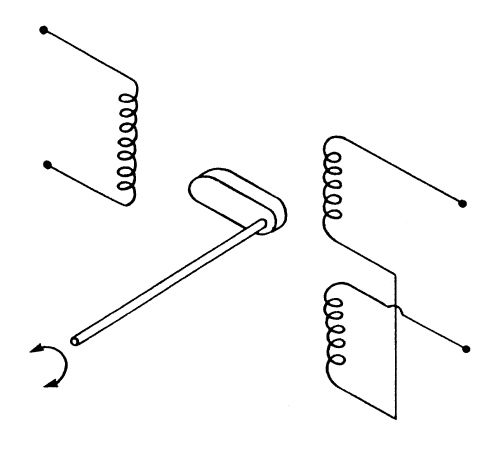
\includegraphics[width=\columnwidth/2]{figures/rvdt.png}
	\caption{Forgó változó differenciál transzformátor elvi rajza \cite{Morris2016b}.}
	\label{rvdt}
\end{figure}

\subsubsection{Lemezes kialakítások}
\label{optarcsa}

A forgás mérésére kialakíthatóak tárcsák, amelyek egy bizonyos jelet tartalmaznak a forgás során. Ezek lehetnek inkrementális kialakításúak, amelyek bizonyos szögelfordulásonként jelet adnak, illetve kódoltak, ahol a kör kerülete mentén kódok elrendezéséből egyértelműsíthető a lemez pozíciója. A technológiák nyújtotta lehetőségekre az optimális kódolási forma a bináris kód, amely 0 és 1 karakterek sorának ábrázolásával kódol különböző egységeket (amelyeket számoknak szokás dekódolni). Jellemző megoldás a Gray kód, amelynek előnye, hogy a kör kerületére felírva két szomszédos körcikk között csak egy helyi-értéken módosul a mintázat, ahogy ezt a \ref{gray} ábra is illusztrálja. 
\begin{figure}
	\centering
	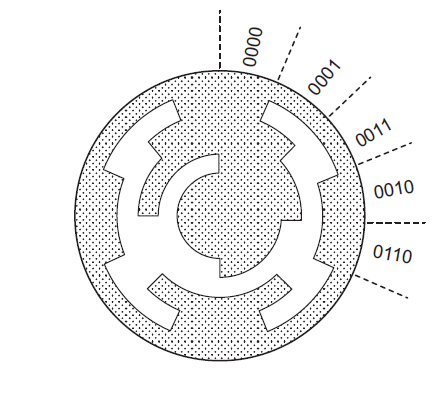
\includegraphics[width=\columnwidth/2]{figures/gray.png}
	\caption{Gray kód megvalósítása tárcsán \cite{Morris2016b}.}
	\label{gray}
\end{figure}
A kódok olvasása történhet \textit{optikai} úton, ahol egy adott szélességen a logikai 1-et kódolja az érzékelés, a logika 0-át pedig, ha nincs jel. Az optikai megoldások lehetnek egyutas, illetve reflexiós szenzorok, amelyeknél áteresztő és takaró, illetve reflektív és elnyelő sávok kódolják a lemez pozícióját \cite{Morris2016b}. Az érintkezés alapú \textit{elektromos elvű} lemezes szenzor vezető és szigetelő szegmensek detektálásán keresztül működik. A lemez egyik oldalán egy alacsony feszültség táplálja, a másik oldalon adott sávokhoz tartozó szénkefék tartoznak, így olvasva külön az egyes cellákat. Az outputok az egyes sávokon olvasott feszültségek alapján magas illetve alacsony között változnak. A végső megoldás \textit{mágneses} elven alapul, amely érintkezésmentes, szennyeződéseknek ellenálló és szélsőséges környezetben is alkalmazható. A lemez hátoldalán tórusz alakú állandó mágnesek helyezkednek el minden olvasandó sáv helyén, ezáltal nagy pontosságot engednek meg. A tárcsán mágnesesen vezető és nem vezető cellákon megy keresztül, vagy áll meg a mágneses fluxus, amelyet a túloldalon található apró tekercsek érzékelnek, ahol szintén magas és alacsony feszültség kódolja a jeleket. A különböző technológiák széleskörű alkalmazásokat tesznek lehetővé, azonban a tárcsás kialakítás limitálja a beszerelhetőséget, valamint a költséget is megnövelik a különböző alkatrészek.

\subsubsection{Rezolver}

A rezolver (angol: Resolver) felépítésre hasonlít egy AC motoréhoz. Két fő alkatrésze egy állórész (sztátor), amelyhez két tekercs tartozik, valamint egy forgórész (rotor), amelyhez tartozhat egy vagy két tekercs is. A szerkezet átmérője általában a 10 és 100 mm között helyezkedik el, amelynek a $0,1\%$-át képes felbontásban elérni. A két alkatrész forgása indukción alapul, a kialakításának sematikus rajzát a \ref{rezolver} ábra mutatja. A két álló tekercs merőleges egymásra, a rotoron található (szinuszosan gerjesztett) tekercselés pozíciója függvényében változik a sztátor tekercseken olvasható kimeneti feszültség.
\begin{figure}
	\centering
	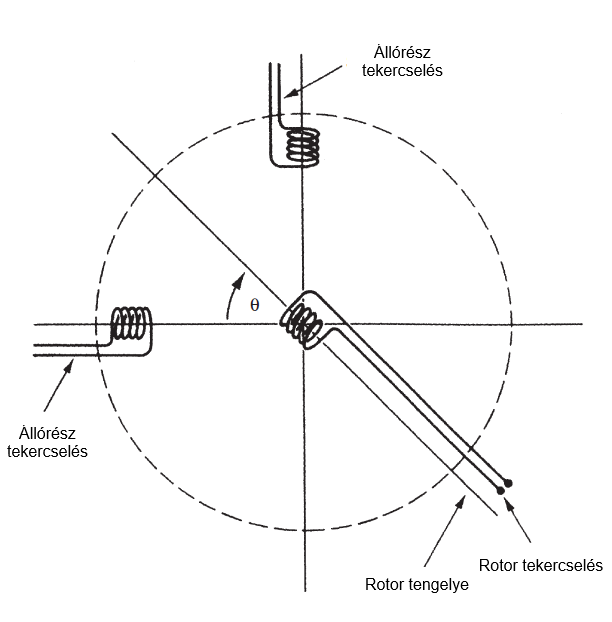
\includegraphics[width=\columnwidth/2]{figures/rezolver.png}
	\caption{Egy tekercses rezolver elvi sematikus ábrája \cite{Morris2016b}.}
	\label{rezolver}
\end{figure}

\subsubsection{Szinkrótranszmitter}

A rezolverhez hasonló elven működik a szinkrótranszmitter (angol: Synchro), vagy rövidebben szinkró. Felépítésében az állórész három tekercse különbözteti meg őket, a rotornak szintén egy vagy két tekercselése bevett a gyakorlatban. A tekercsek a kör kerületén egyenlően elosztva, $120\degree$-t zárnak be egymással, ez az aszimmetrikus tekercselés a felbontás megnövekedését eredményezi, ami $0,5\%$-ot jelent. A szinkró egymagában képes elfordulást mérni, de egy gyakrabb alkalmazásában párban használják, a \ref{selsyn} ábrán látható kapcsolásban, nemcsak pontosabb elfordulásmérést eredményez, de akár érintkezésmentes adatátvitelre is képes. Ennek a szerkezetnek a neve Selsyn-transzmitter, amelyben a két rész elnevezése szinkrótranszmitter és szinkrótranszformátor. A transzformátor álló rotorján adott bemeneti feszültség által indukált mágneses tér, az összekapcsolt sztátorokon keresztül megjelenik a transzmitter rotorján, ahol ugyanazt a szinuszos feszültséget tudjuk mérni, egy fáziseltolással, amely egyenlő a két rotor közötti szöggel. Így alkalmazható információátvitelre a Selsyn, akár nagyobb távolságokon keresztül is.
\begin{figure}
	\centering
	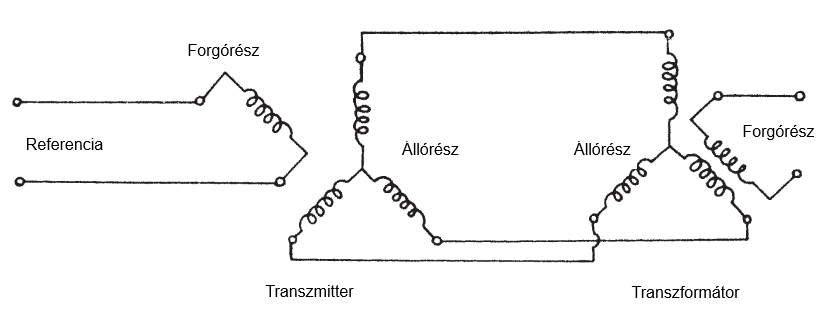
\includegraphics[width=\columnwidth*8/10]{figures/selsyn.png}
	\caption{A Selsyn-transzmitter elrendezése \cite{Morris2016b}.}
	\label{selsyn}
\end{figure}

\subsubsection{Forgó Induktoszin}

Az elfordulásmérésre alkalmazható induktoszin a lineáris változatához (\ref{linind} szekció) hasonló elven, eltérő kialakítással működik. A szenzor egy rotor és egy sztátor oldali tárcsából áll, amelyeken két négyzethullám alakú szál megy végig a felületükön. A tárcsák átmérője általában 75 és 300 mm közé esik, és 0,05 szögperc felbontással rendelkezik, azonban a lineáris induktoszinhez hasonlóan a mérési tartománya rendkívül rövid, így egy segédmérőeszközre van szüksége a működéshez.

\subsubsection{Giroszkóp}
\label{lingiro}

A giroszkópok a szögelfordulás valamint a szögsebesség mérésére is egyformán alkalmasak, megvalósításuk lehetséges mechanikus és optikai úton is, azonban itt az elfordulás mérésére alkalmas szenzorok lesznek tárgyalva, a szögsebességet mérő giroszkópok egy későbbi fejezetben kerülnek ismertetésre. 

A \textit{mechanikai} giroszkóp fő alkatrésze egy motorral meghajtott nagy impulzusmomentummal rendelkező kerék, amely a forgástengelyt a perdületének köszönhetően állandó helyen tartja, így referenciaként tud működni. A szenzor külső szerkezete van hozzáerősítve a mérendő testhez, a kimenet pedig a rögzített keret a kerék forgástengelyének hajlásszögének mértéke lesz. A szögelfordulás mérésére kétféle kialakítás létezik, a szabad- és integráló giroszkóp (angol: free, rate-integrating/integratin gyroscope). A szabadon mozgó mechanizmus közvetlen elfordulás mérésére képes, két merőleges tengelyen, amely két tekercsel ellátott keret alkalmazásán keresztül történik. A szerkezet sematikus ábráján láthatjuk ezt a kialakítást (\ref{freegyro} ábra). 
\begin{figure}
	\centering
	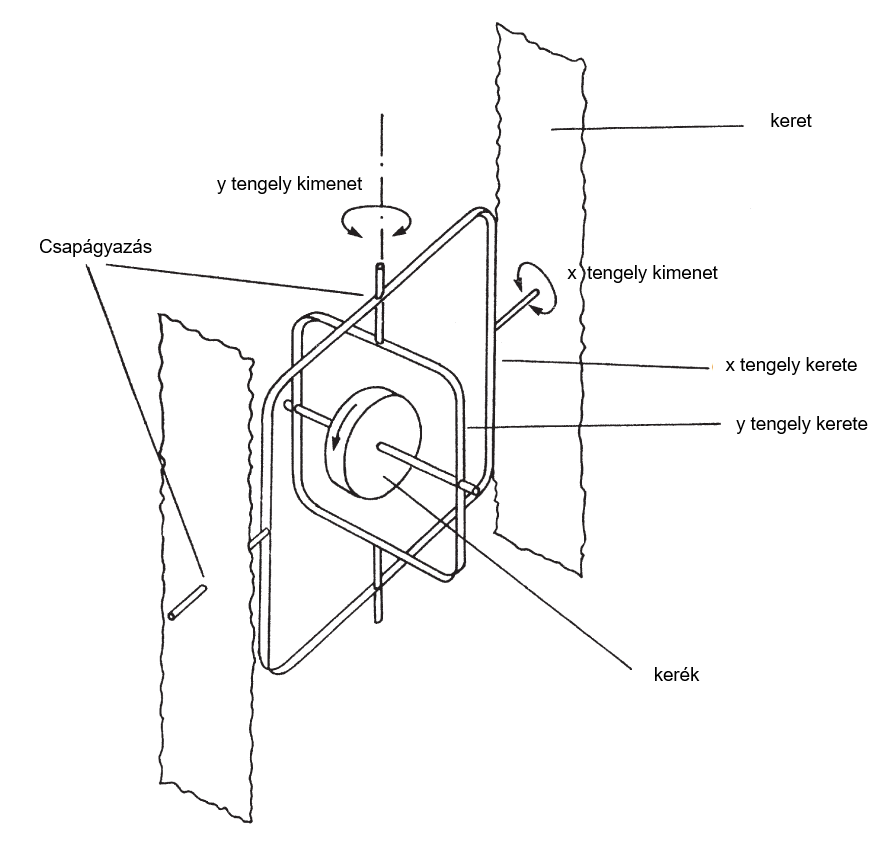
\includegraphics[width=\columnwidth/2]{figures/freegyro.png}
	\caption{A szabadon mozgó giroszkóp kialakításának sematikus rajza \cite{Morris2016b}.}
	\label{freegyro}
\end{figure}
A kerék forgatómotorja csúszógyűrűn keresztül kap áramot, valamint a csapágyazás is itt történik. A szabad kialakítás $10\degree$-os tartományban működik jó pontossággal a tekercsek kiterjedése miatt, azonban a szenzor újraindításával más tartományban is mérhetünk pontosan a kerék forgásának beállása után. Másik hátrány az idővel fellépő szögeltolódás (precesszió), amely akár $0,5\degree$ mérési hibát is eredményezhet, mivel ez a pontatlanság sok alkalmazást kizár, az integráló giroszkóp nagyobb népszerűségnek örvend. A kialakítás elvi felépítése hasonló, azonban csak egy tengely elfordulását méri, így csak egy kerettel és tekercsel rendelkezik. A szögsebességből történő integrálással a precesszió áthidalható, így pontosabb eredményt ad hosszabb távon mint a közvetlen szögelfordulást mérő mechanizmus \cite{Morris2016b}.

Az \textit{optikai} giroszkópok közül az elfordulásmérésre kialakított szerkezet gyűrűs lézer giroszkópnak nevezik. Egy üveg-kerámia háromszög alakú kamrában hélium-neon gáz elegye van, amelyben egy anód két katóddal generál két ellenkező irányú lézersugarat, amelyek a háromszög sarkaiban található három tükör szabályoz. A szerkezet bármekkora forgása során a lézersugarak útjának hossza megváltozik, így a két sugár fáziseltolódását okozva (Sagnac-effektus), amelynek mérésével kiszámítható az elfordulás szöge. A lézeres giroszkóp ezért lényegesen pontosabb, a kialakítása kompaktabb, mint a hasonló költségű mechanikus giroszkópok \cite{Morris2016b}.

\subsection{Szögsebesség mérése}

A szögsebesség vagy fordulatszám mérés a közvetlen megoldás az eredeti alkalmazáshoz, a fordulatszámok összehasonlításához. Előfordulnak a \ref{elmozd} és \ref{elford} fejezetekben bemutatott, lineáris illetve forgó mozgás mérését alkalmazó, vagy továbbfejlesztő technológiák, valamint kizárólag sebességmérésre alkalmas szenzorok \cite{Morris2016b}.

\subsubsection{Digitális fordulatszámmérők}

A digitális fordulatszámmérők, avagy tachométerek általában kontaktus nélkül működnek, és jelzőket érzékelnek, amik egy forgó palástfelületen vagy tárcsán egyenlően vannak elosztva, amely a mérés felbontását adja. Változatos típusú érzékelési elv alapján mérnek, és jelzőnként egy elektronikus impulzust továbbítanak egy számlálónak. A fordulatszámot a jelek száma és egy időegység hányadosaként adják, így valójában átlag sebességet mérnek. 

Az \textit{optikai} fordulatszámmérőkben az optikai impulzusokat kétféle módszerrel lehet generálni, a tárcsás elfordulásmérőkhöz hasonlóan. Az első elrendezésben a tárcsákon egymástól egyforma szögtávolságra ablakok helyezkednek el, amelyek magasságában a tárcsa egyik oldalán egy fényforrás, másikon egy szenzor található. A második elrendezésben a szenzor és a fényforrás azonos oldalon helyezkedik el, az ablakok helyett pedig reflektív sávok vannak a tárcsa felületén. A fényforrások általában lézerek vagy LED-ek, míg a detektorok feladatát fotodiódák vagy fototranzisztorok látják el. Az optikai fordulatszámmérők pontosságukban elöl járóak, azonban a szennyeződéseknek való kitettségük miatt sok esetben nem alkalmazhatóak \cite{Morris2016b}.

Az \textit{induktív} fordulatszámmérők, más néven változó reluktanciájú sebességérzékelők (variable reluctance velocity transducer) egy széles körben főleg a járműiparban használt digitális szenzorok. Az érzékelő egy pólusainál elhegyesedő állandó mágnes köré erősített tekercs. A pólusok előtt elmozduló ferromágneses testek a mágneses tér megváltoztatásával a tekercsben feszültség indukálódik, ami a szenzor kimeneteként szolgál. Egyszerűbb kialakításokban egy ferromágneses fogaskerék elmozduló fogai közeledésének és távolodásának hatására változik a mágneses fluxus, a változás sebessége pedig arányos lesz az indukált feszültség amplitúdójával. A kimenet ezáltal pozitív és negatív impulzusokból áll, a jel frekvenciája pedig megfeleltethető a fogaskerék szögsebességével \cite{Morris2016}. Egy bonyolultabb kialakítást látunk a \ref{vrt} ábrán, ahol egy kompozit tárcsába a kerületen egyenlő távolságban vas rudak vannak behelyezve. Ahogy a vas betétek a mágnes felé mozognak növekszik a mágneses fluxus, távolodásukban pedig csökken, a mérés pedig a fogaskerékhez hasonlóan zajlik. A legnagyobb mérhető fordulatszám nagyjából $10\,000$~rpm (rotations per minute, percenkénti fordulatok száma), az impulzusok adott vastagsága miatt, amely túl nagy sebesség esetén az impulzusok egybefolyását eredményezi. Az optikai úton való mérésnek itt előnye van, mivel az impulzusok vékonyabbak, így magasabb fordulatszámok mérésére is alkalmas, a fogaskerék mérése pedig csak alacsonyabb fordulatszámokat enged meg a produkált jelek életlensége végett.
\begin{figure}
	\centering
	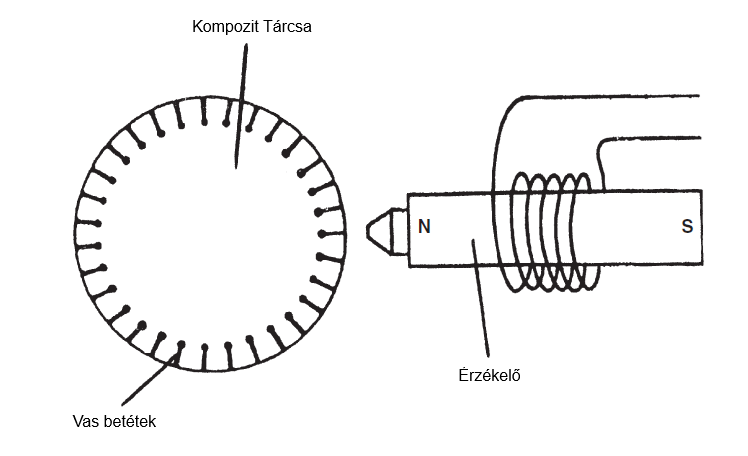
\includegraphics[width=\columnwidth*8/10]{figures/vrt.png}
	\caption{Változó reluktanciájú sebességérzékelő elvi rajza \cite{Morris2016b}.}
	\label{vrt}
\end{figure}

A \textit{mágneses} fordulatszámmérők egy Hall-effektus szenzort alkalmaznak, amelynek működése a \ref{linind} szekcióban bemutatásra került. A mérőeszköz egy fogaskerék vagy hasonló fogazott tárcsa mérésére alkalmas, amely egy állandó mágnessel zár közre egy Hall-effektus szenzort. Amikor egy fogárok van a szenzor előtt a teljes mágneses tér keresztül megy a szenzoron, azonban ha a fog közeledésével eltereli a mágneses tér egy részét, így annak hatása csökkenni fog. Ezáltal a szenzor a forgás sebességével arányos frekvenciájú feszültséget fog kimenetére adni.

\subsubsection{Stroboszkópos mérőeszközök}

A stroboszkópos szögsebesség mérés elgondolása hasonló a digitális szenzorokéhoz, azonban az impulzusok elektromosan gerjesztett fények, amelyek a kerületen időközönként ismétlődő elemekről visszaverődve adnak jelet. Ezek az elemek lehetnek természetesen előforduló geometriák, mint a fogaskerék fogai, vagy mesterségesen előállított tulajdonságok, például fekete és fehér színű sávok az eszköz felületen. A stroboszkóp frekvenciája változtatható, így azt szinkronizálni lehet a megjelenő jelek frekvenciájával. Ha a két frekvencia megegyezik, a felületen megvilágított elem megjelenésében állónak tűnik. A megfelelő frekvencia megtalálásához azonban a harmonikusok kizárása szükséges, amit az eredeti frekvencia többszöröseinek vizsgálatával lehet megtenni, így a legnagyobb hullámhosszú mérhető harmonikust megtalálva. Ennek a szenzornak gyakori kialakítása a kézben hordozható kivitel, ugyanis a stroboszkóp precíz pozicionálására nincs szükség. A stroboszkópos fordulatszámmérők mérési tartománya $110 - 150\,000$~1/perc, és $\pm1\%$ hibával operál \cite{Morris2016b}.

\subsubsection{Analóg fordulatszámmérők}

Általánosságban az analóg fordulatszámmérők kevésbé pontosak mint digitális változataik, azonban sok alkalmazásra teljes mértékben megfelelnek.

A \textit{DC - egyenáramú} tachométer a forgás sebességéhez nagyjából illeszkedő feszültségkimenetet produkál. A felépítése hasonlít az egyenáramú generátoréhoz, egy statikus állandó mágnes keretből és egy tekercselt csúszógyűrűn keresztül táplált forgórészből áll. A generátorral ellentétben a mérési pontosságra helyezkedik a hangsúly, így például a rotor súlyának csökkentése miatt egy üreges üvegszál adja a tekercs belsejét. A kimeneti feszültség nagyjából minden $1\,000$~rpm változásnál $5$~V feszültségkülönbséget ad le (a forgás iránya a feszültség előjeléből látszik), így nagyjából $0-6000$~rpm egy tipikus mérési tartomány. A szenzor problémája, hogy arra alkalmas esetekben megjelenhet váltóáramú búgófeszültség (az egyenáram váltóáram szerű feszültség ingadozása) a kimeneti jelen, aminek amplitúdója nagyjából feszültségérték $2\%$-át teszi ki.

A \textit{AC - váltakozó áramú} fordulatszámmérők hasonlóan az egyenáramú megfelelőjének a szögsebességgel arányos feszültségkimenetet generálnak. A kialakításuk egy kétfázisú indukciós motorra hasonlít, két sztátor tekerccsel és általában egy úgynevezett csészeforgórésszel, amelyet a \ref{actach} ábra mutat be. 
\begin{figure}
	\centering
	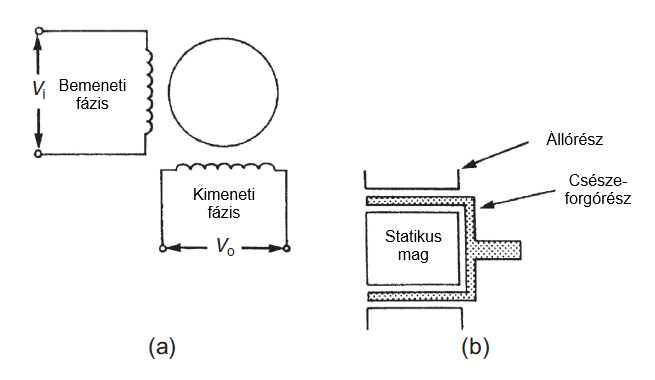
\includegraphics[width=\columnwidth*7/10]{figures/actach.png}
	\caption{Váltóáramú tachométer: (\textbf{a}) tekercsek elrendezése; (\textbf{b}) Álló és forgórész sematikus ábrája \cite{Morris2016b}.}
	\label{actach}
\end{figure}
Az állórész egyik tekercsét váltóáram táplálja, a kimenetet pedig a másik merőleges tekercsben indukált feszültség lesz. A rotor állásakor ez a feszültség zérus, és a fordulatszám növekedésével arányosan fog a feszültség amplitúdója is növekedni. A forgásirány változása a kimeneti feszültség $180\degree$-os fáziseltolódásából lehet látni, így mind a kimenet fázisa, mind az amplitúdója is fontos a mérés szempontjából. Általában a mérési tartomány $0-4000$~rpm, a mérési hiba pedig a teljes skála $\pm0,05\%$-át teszi ki. Léteznek költséghatékonyabb, kalickás rotoros kialakítású szenzorok is, azonban ezeknél a mérési hiba $\pm 0,25\%$ körül mozog.

Az úgynevezett \textit{csészeforgórészes}, vagy \textit{örvényáram} fordulatszámmérők esetén, egy központi orsón elhelyezett állandó mágnes egy nem mágnesezhető csésze borítja, amely egy elektromosan vezető hengerpalástból áll, ahogy a \ref{dragcup} ábra mutatja.
\begin{figure}
	\centering
	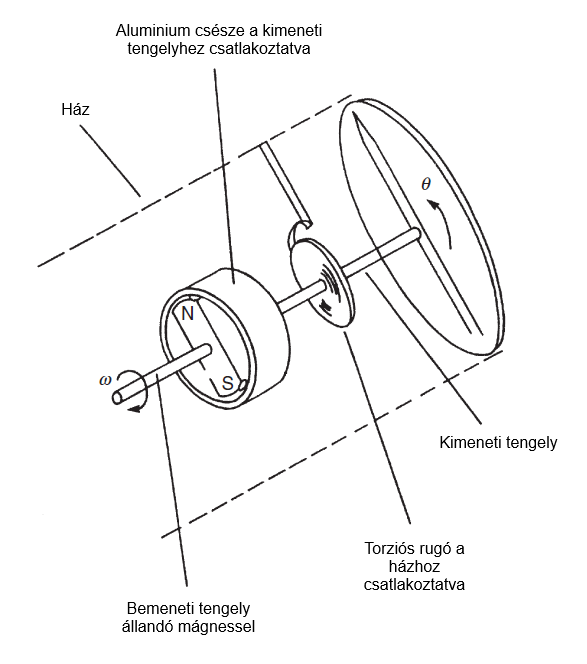
\includegraphics[width=\columnwidth*6/10]{figures/dragcup.png}
	\caption{Örvényáramos fordulatszámmérő elvi rajza \cite{Morris2016b}.}
	\label{dragcup}
\end{figure}
Az orsó forgásával a csészében örvényáramok keletkeznek, amelyek az állandó mágnes által indukált mágneses térrel kölcsönhatásba lépve nyomatékot generálnak. Ez a forgatónyomaték addig forgatja az orsót, ameddig a rajta található torziós rugó nyomatékával kiegyenlítődnek. A nyomatékkiegyenlítődés állapotában a csésze szögelfordulása arányos az orsó és a mágnes fordulatszámával, így ez adja a szenzor kimenetét. Általában a mérési hiba $\pm 0,5\%$ körül mozog, a mérési tartomány pedig $15\,000$~rpm is lehet \cite{Morris2016b}.

\subsubsection{Szögsebesség mérő giroszkópok}

A \textit{sebességérzékelő} giroszkóp (angol: rate gyroscope) közel azonos felépítéssel rendelkezik, mint a \ref{lingiro} fejezetben tárgyalt integráló giroszkóp, azzal a különbséggel hogy egy torziós rugóval egészül ki, ezzel limitálva a keret forgómozgását, ahogy a \ref{rategyro} ábra is mutatja. A szenzor abszolút szögsebességet mér, gyakran jelek stabilizálására alkalmazzák navigációs rendszerekben. A felbontása $0,01\frac{\degree}{s}$, a mérési tartománya $50\frac{\degree}{s}$-ig terjed.
\begin{figure}
	\centering
	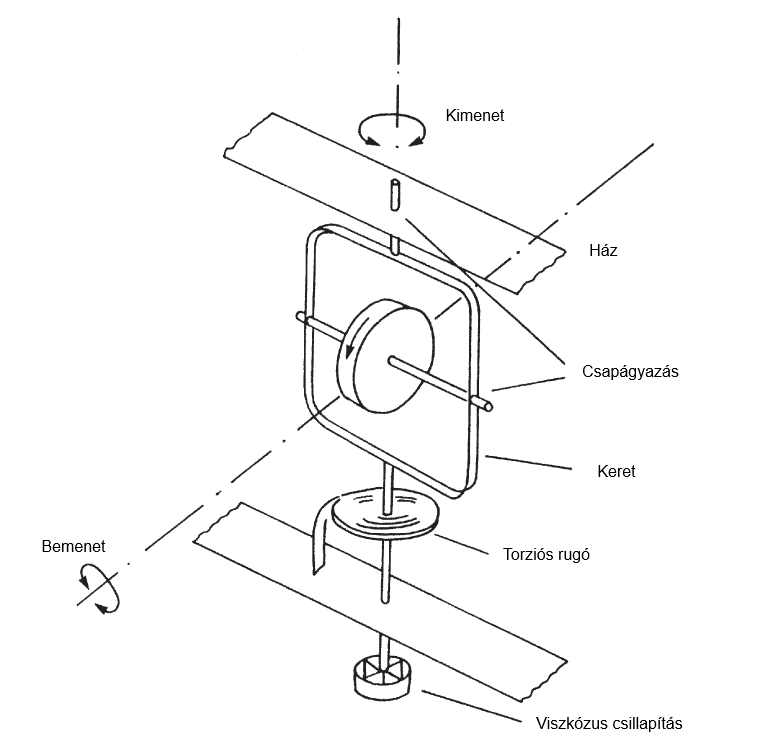
\includegraphics[width=\columnwidth*5/10]{figures/rategyro.png}
	\caption{A sebességérzékelő giroszkóp sematikus ábrája \cite{Morris2016b}.}
	\label{rategyro}
\end{figure}
Az \textit{optikai szálas} giroszkóp egy viszonylag új szenzortechnológiai eszköz. A fényforrásból származó sugarak a beeséskor kettéválasztódnak, majd a feltekercselt optikai szál két végébe vezetődnek. A tekercsbe ellenkező irányban haladnak, majd a tekercs ellentétes végén jelennek meg. A nyalábosztó egyesítve az így kilépő két sugarat egy interferométerbe irányítja azokat. A mérés során a két nyaláb fáziseltolódásának detektálása történik, amely a tekercs elfordulásával keletkezik, és annak mértékével arányos \cite{Morris2016b}.

A \textit{MEMS} giroszkóp, vagyis a mikro-elektromechanikai rendszert alkalmazó (Microelektromechanical System) szenzorok már széles körben alkalmazva vannak a szögsebesség méréséhez, ezzel szemben az elmozdulásra még nem fedeztek fel alkalmazható MEMS kialakítást. A tipikus elrendezése egy ilyen szenzornak a \ref{memsgyro} ábrán látható. 
\begin{figure}
	\centering
	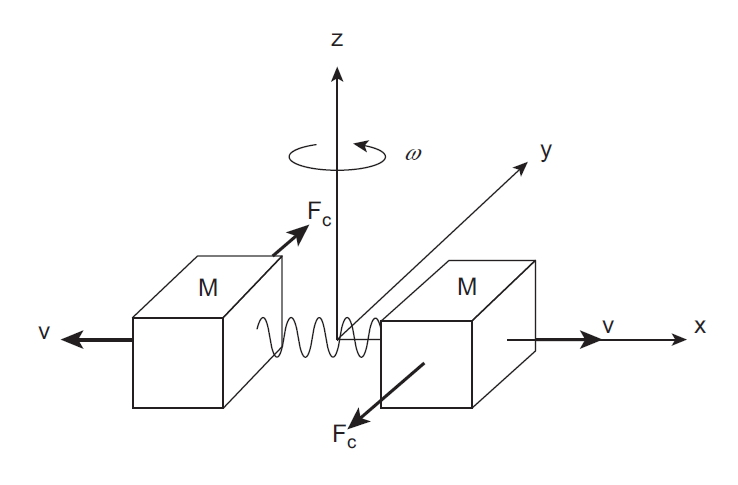
\includegraphics[width=\columnwidth*7/10]{figures/memsgyro.png}
	\caption{Egy MEMS giroszkóp általános elrendezése \cite{Morris2016b}.}
	\label{memsgyro}
\end{figure}
A szenzor két egyforma $M$ tömegű fém testből áll, amelyek szimmetrikusan oszcillálnak, vagyis mindig egymással ellentétes irányban mozognak. Amikor a tömegekre $\mathbf{\Omega}$ szögsebesség jelenlétében $\mathbf{F}$ Coriolis-erő hat, amelynek mértéke a következőképpen adódik: $\mathbf{F}=-2M\mathbf{\Omega}\times \mathbf{V}$, ahol $\mathbf{V}$ a súlyok aktuális sebessége. Mivel a tömegek a forgástengely két oldalán vannak, így a Corialis-erők ellentétes irányban, az oszcillációra merőlegesen mozdítják el a tömböket, így megnövelve a közöttük lévő távolságot. Ezáltal a fém súlyok közötti kapacitás megváltozik, amely arányos lesz az $\mathbf{\Omega}$ szögsebesség értékével. A kapacitásváltozás értéke mind analóg, mind digitális jellé is konvertálható, a giroszkóp kimeneti jelét adva. A MEMS rendszerekről általában, így a giroszkópról is elmondható, hogy a gyártási költsége és energiafogyasztása alacsony, emellett nagy pontossággal operál. Ezen felül bármilyen lineáris mozgásra teljes mértékben érzéketlen, mivel a tömegek egyszerre mozognak bármilyen irányba történő erőhatásra, a relatív elmozdulásuk nélkül pedig a kapacitás fog változni. A mérési tartományuk akár $2700\,\frac{\degree}{s}$ is lehet, azáltal nem meglepő, hogy széles körben alkalmazzák, kamerák stabilizálásától, járművek elfordulásán át, az autók felfordulásának jelzéséig. 

\subsection{Szöggyorsulás mérés}

A szögsebesség mérésére alkalmas lehet egy gyorsulásmérő eredményeit integrálni, amely elfogadható eredményekkel rendelkezik, hiszen az integrálás folyamata csökkenti is a mérési zajt. A sebességmérésre azonban mégsem egy elterjedt mérési módszer, mivel az integrálás során egy átlagsebesség számolására kerül sor, egy adott intervallumban, amely nem kielégítő, hogyha egy pályán folyamatos sebességadatra van szükségünk \cite{Morris2016b}. Szintén nagy hátránya az integrálásnak, hogy megjelenik egy 'offset' (eltolás) jellegű hiba ("drift"), amely folyamatosan kumulálódik, és az integrálásból következik, így kiküszöbölhetetlen.

A szöggyorsulás mérésének alapját (a lineáris gyorsulás méréséhez hasonlóan), egy forgó tömeg adja, amely a külső, forgó testhez erősített házhoz van rögzítve. Az elfordulás következtében a tömegben forgatónyomaték fog ébredni, amely egy torziós rugó és egy csillapítás összegével lesz kiegyenlítve, ahol a rugón keresztül lehetséges kimenetet felvenni, a csillapítás feladata pedig a rezgések kiszűrése. 

%----------------------------------------------------------------------------
\section{Vezérlés eszközei}
%----------------------------------------------------------------------------

A szenzorokból érkező jeleket, általában feszültséget egy adatfeldolgozó eszközben kezeljük. Ugyanezek az eszközök képesek kell legyenek a kimenő jel adására is, visszajelző eszközök irányítására. Ezek az eszközök általában ipari folyamatok automatizálására, gépek ki- és bekapcsolására alkalmas relék és azok rendszereinek digitalizálásával jöttek létre. Egy másik megközelítés a számítástechnika fejlődésével, az áramkörök méretének csökkenésével tört előre, ugyanis az ilyen apró számítógépek számos szabályozási feladat elvégzésére lettek képesek. Ebben a fejezetben a legnépszerűbb, jelen felhasználásra leginkább alkalmazható hardver- és szoftverrendszerek kerülnek bemutatásra, amelyek már az iparban fennálló technológiák és támogatásuk is, segédanyagaik széles körben elérhetőek.

\subsection{Ipari vezérlők}

\subsubsection{PLC}

A \ref{plckep} ábrán látható egy programozható logikai vezérlő (PLC: programmable logic controller), az ipari automatizáció kulcsfontosságú eszköze. Az ipari automatizációban eleinte elektronikus relékből és tekercsekből, kábelekkel összekötött áramköröket használtak. A PLC ötlete egy a relék kapcsolási rajza alapján létrehozott programozási nyelv (Létra Diagram) implementálása egy hardverre, amely ezáltal újraprogramozható, és az alapján alkalmas a ki- és bemenetek (I/O: Input/Output) közötti kapcsolat megalkotására. A modern PLC-k emulálják a elektornikus létra diagramok viselkedését, azonban fizikailag már csak a be- és kimenetek vannak megépítve. Az ilyen rendszerek előnye, hogy modulárisak, a I/O-k, kommunikációs technikák, platformok cserélhetőek és bővíthetőek, így pont akkora rendszer alakítható, amekkorára szükség van, ezáltal költséghatékony is lesz. Az ipari környezetre való tekintettel ezek a rendszerek ellenállóak a környezeti behatásoknak, hőmérsékletnek, ütéseknek, por- és olajszennyeződésnek, valamint robusztusak, a hibáik ellen védőrendszerek vannak beépítve, ezáltal megbízhatóak. A programozásuk is relatív (a mikrovezérlőkhöz képest) könnyen tanulható, logikusan, intuitívan felépített. Az ember-gép kapcsolat kialakításához sok esetben egy kis méretű kijelző jelzi a program állapotát, indikátorfények is gyakran segítik a hibaelhárítást. A PLC-k egyes moduljai végzik ezeket a feladatokat, amelyek a következő felosztásban találhatóak meg \cite{Alphonsus2016}:
\begin{itemize}
	\item \textbf{Keret/Ház}: A modulok fizikai összetartására, és elektronikus kapcsolatának megteremtéséhez alkalmazzák az egész PLC hardverének tárolóegységét.
	\item \textbf{Tápegység}: A külső feszültségforrás (általában 24 V, DC) mindegyik másik modulhoz eljuttatása a feladata, kisebb rendszerek esetén az irányított eszközöket is táplálhatja, azonban nagy készülékek esetén általános a külső DC vagy AC forrás.
	\item \textbf{Programozó felület}: A programok összeállítását és futtatását megvalósító modul. A visszajelzés függhet a gyártótól és kiviteltől, de általában indikátorok és kristályos vagy LED-es kijelzők végzik ezt a feladatot, a bevitel lehet egy pár speciális gomb, vagy akár egy billentyűzet is. Gyakori a külső számítógéppel vagy laptoppal való kapcsolat is, így a felprogramozás és hibajavítás egy külső eszközön történik a kommunikációs platformon keresztül.
	\item \textbf{Ki-/bemeneti szakasz}: Az összes irányítandó eszközhöz való kapcsolatot, valamint a processzorral való kommunikációt ez a modul valósítja meg, ezáltal a két rendszer működési feszültsége közötti konverziót, és a galvanikus leválasztást is feladata elvégezni. A be- és kimenetek lehetnek fixek, amelyek akár a processzor modulba beépítve már biztosítva vannak, valamint léteznek moduláris szakaszok is, amelyek a specifikus, követelményeknek megfelelően bővítik a rendszert. A ki- és bemenetek lehetnek digitálisak, amelyek ki- és bekapcsolás között változnak, vagy analógok, amelyek két határ közötti feszültséggel biztosítják egy szenzor jelét, vagy kivitelezik az irányítási feladatot.
	\item \textbf{Processzor modul}: A szabályozás elengedhetetlen és alapvető komponense, itt valósul meg a számítások elvégzése, a memória kezelése és a többi komponens irányítása. A modul integrált áramköri chipekből áll: a mikroprocesszor, amely a matematikai műveleteket végzi, a memória, a program és a változók tárolására, valamint a kettő közötti kommunikációt végző áramkörök.
\end{itemize}
\begin{figure}
	\centering
	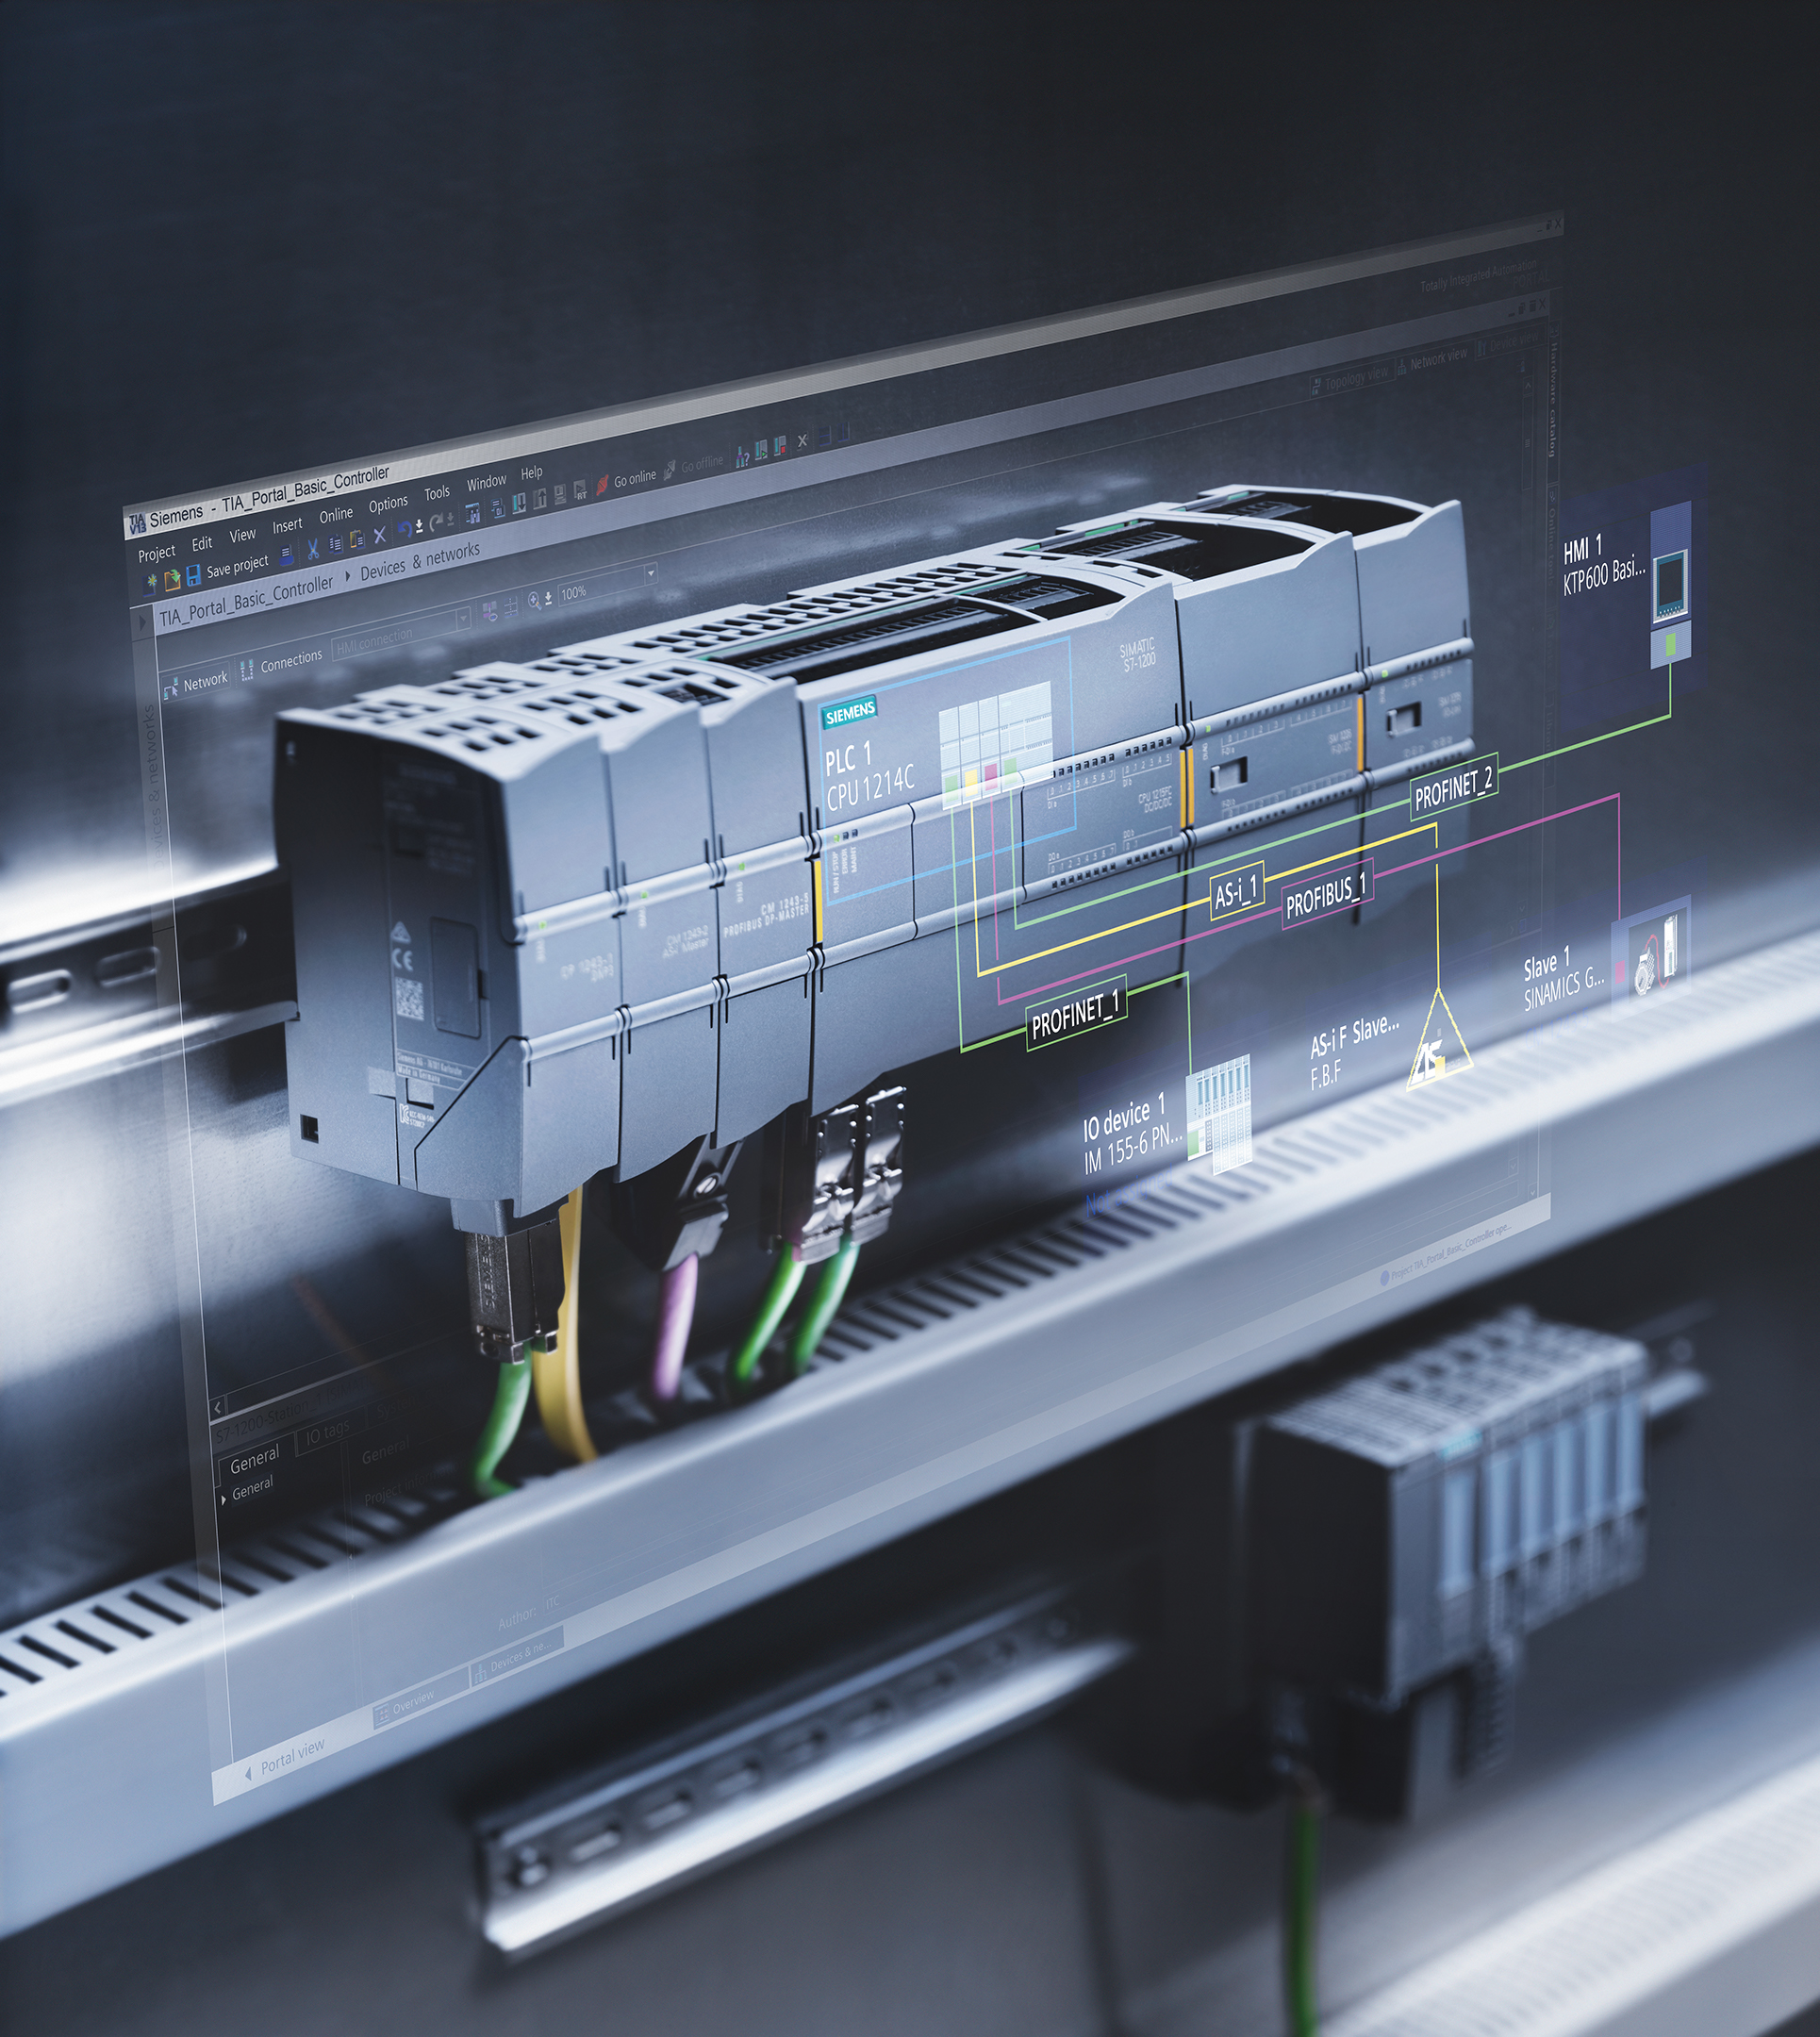
\includegraphics[width=\columnwidth*5/10]{figures/siemens_plc.jpeg}
	\caption{Siemens Simatic S7-1500 PLC. forrás: \cite{siemens_plc}}
	\label{plckep}
\end{figure}
A PLC-k működtetésére több programnyelvet is alkalmaznak, melyek az IEC Standard 1131-3 szabványban vannak rögzítve, ez az öt nyelv a legtöbb gyártó által támogatott nyelveket lefedi \cite{Baresi1998}: 
\begin{itemize}
	\item \textbf{Utasítás Lista (IL: Instruction List)}: Egy alacsony szintű, Assembly-re hasonlító programozási nyelv, vagyis rövid szöges kódok sorai. Az instrukciós lista jól alkalmazható lineáris, kis feladatok optimális kóddal való megoldására, azonban strukturált programok létrehozására nem képes. Az IL interpretálására általánosságban az összes PLC képes, így általában ez az a kód amivé lefordítódik az összes többi programozási nyelv \cite{Baresi1998}.
	\item \textbf{Strukturált Szöveg (ST: Structured Text)}: Magas szintű, blokk szerkezetű nyelv, amely a Pascal programozási nyelvre alapul, így sok elemet onnan merít. Adattípusokat alkalmaz, és támogatja a strukturált programozást, ezért szokták az \textit{új PLC programozási nyelvnek} hívni, hiszen alkalmas a modern programozás komplexitásának és modularitásának kivitelezésére \cite{Baresi1998}.
	\item \textbf{Létra Diagram (LD: Ladder Diagram)}: A leggyakrabban használt, már említett programozási fajta, a relé kapcsolásokat digitalizáló nyelv \cite{Dey2020}. Népszerűségét a könnyen tanulhatóságának, egyszerűségének köszönheti, azonban komplex rendszerek és programok kivitelezésére alkalmatlan.
	\item \textbf{Mnemonikus Instrukció (MI: Mnemonic Instructions)}: A létra diagramból kinyerhető gépi szintű utasításokat tartalmazó kód, közvetlenül a mikroprocesszorral kommunikál. Ez nem része a szabványosított programozási nyelveknek, ugyanis a programot az LD fordító készíti el \cite{Dey2020}.
	\item \textbf{Funkcióblokk Diagram (FBD: Function Block Diagram)}: Ez egy grafikus nyelv, amely a jeleket és adatokat blokkok között továbbítja, így modulárissá és újrahasználhatóvá téve a kódokat. A funkcióblokkok egyszerű kódokat kiviteleznek Strukturált Szövegben megírt rendszerekkel, amelyek legtöbbször áramköri elemeket, döntéseket akár késleltetéseket valósítanak meg \cite{Baresi1998}.
	\item \textbf{Szekvenciális Funkciós Diagram (SFC: Sequential Function Chart)}: Szintén egy grafikus nyelv, amely a belső szerkezet rendszerezésére használható. A PLC folyamatait lépések és azok közti átmenetekké formálja, amelyeken belül általában LD programok futnak. Az átmenetek valamilyen feltételek, döntéseket valósítanak meg, a lépések pedig a akciók kivitelezését végzik.
\end{itemize}
\subsubsection{Programozható Relék}

A programozható relék (Programmable/'Smart' Relay) a PLC kialakításából kifejlődött, kompakt, kis ki- és bemenetszámú logikai vezérlők. Ezek az eszközök akár önmagukban is alkalmazhatók, általában kevés modullal, I/O bővítő és kommunikációs platform szakaszokkal rendelkeznek. Előnyük, hogy széles tápfeszültséggel képesek operálni (24-240 V váltóáram, 12-24 V egyenáram), kis rendszereket hatékonyan tudnak működtetni, és a PLC rendszerekhez képest is költséghatékonyak \cite{zeliologic_catalog}. Programozásuk a gyártó natív szoftverében történik -- általában létra diagram (LD) vagy funkciós blokkdiagram (FBD) nyelveken --, gyakran internetes vagy felhőalapú kommunikációra képesek, illetve egyes modelleknél külső tárolók (SD kártya) behelyezésével is lehetséges a felprogramozás.

\subsection{Mikrovezérlők}

Az első hivatalos mikrokontroller az Intel gyártmánya volt, azonban előtte is volt már hasonló alkalmazásra igény. A Texas Instruments számológép áramkörei kiszélesítették piacukat, és már 1971-ben hirdetve voltak mint pénztárgép, óra és mérőrendszer alkatrészek. Napjainkban a mikrovezérlők már széles körben megtalálhatóak, háztartási eszközökben, telekommunikációban, járművekben, akár a gyártás automatizálásában is. A mikrovezérlők általában egy alacsony feszültségű nyomtatott áramkörök, amelyek képesek egy mikroprocesszor alkalmazásával: be-/kimenetek és perifériák kezelésére, időzítők és adatok eltárolására, és ezáltal komplex rendszerek üzemeltetésére \cite{Gridling2007}. Ezeknek a feladatoknak ellátásához, az egyes elemek irányításához az alábbi részelemek szükségesek:
\begin{itemize}
	\item \textbf{Processzor}: A vezérlő központi feldolgozó egysége (CPU). Az aritmetikai-logikai egység, a vezérlőegység és regiszterek (közeli memóriák) alkotják, amelyek közös munkája az összes számítás, irányítás kivitelezése.
	\item \textbf{Memória}: A memória általában két részre van osztva, program- és az adatmemóriára. Nagyobb vezérlőkben az úgynevezett Direkt Memória Hozzáférés vezérlő (DMA: Direct Memory Access) irányítja a perifériák és a memória közötti kommunikációt, a processzor helyett, így gyorsítva mindkét rendszert.
	\item \textbf{Programmegszakítás vezérlő (Interrupt Controller)}: A programmegszakítások külső vagy belső események esetén következnek be, amelyek a normál programmenetet félbeszakítják, és végrehajtják az esemény kezeléséhez szükséges programrészt. A különleges események várakozásának csökkentésére, valamint az energia megtakarításra alkalmasak.
	\item \textbf{Időzítők/Számlálók}: A legtöbb vezérlő rendelkezik legalább egy, de általában 2-3 számlálóval. Ezek használhatóak események időzítésére, időintervallumok mérésére, vagy események számlálására.
	\item \textbf{Digitális Ki-/Bemenetek}: Párhuzamos digitális ki- és bemeneti "kapuk", vagy portok a mikrovezérlők egyik fő funkcionalitásai. Az I/O lábak, tüskék száma 3-4-től akár 90-ig is terjedhet, a vezérlő családtól és modelltől függően.
	\item \textbf{Analóg Ki-/Bemenetek}: A legkisebb vezérlőkön kívül, a mikrovezérlők általában rendelkeznek analóg/digitális konverterekkel, amelyek változó darabszámban (2-16) és felbontással (8-12 bit) jelennek meg. Általában analóg összehasonlító áramköröket is tartalmaznak a mikrovezérlők, néhány esetben előfordul a digitális/analóg konverterek alkalmazása, amelyekkel a digitális jelekből analóg kimeneteket lehetséges előállítani.
	\item \textbf{Interfészek (Interfaces)}: A vezérlők általában rendelkeznek legalább egy soros interfésszel, amellyel a felprogramozó számítógéppel kommunikálnak. Soros portok a perifériákkal való kommunikációban is részt vehetnek, a legtöbb mikrovezérlő esetében több interfész is rendelkezésre áll, mint az SPI (Serieal Peripheral Interface) vagy SCI (Serial Communications Interface) protokollok. Rendszerint található a mikrokontrollereken buszos kommunikáció, IIC/I2C (Inter-Integrated Circuit) és CAN-busz (Controller Area Network) kommunikációs protokollok jelentkeznek többségében. Egyéb jellemzően alkalmazott interfészek lehetnek még a PCI (Peripheral Component Interconnect), az USB (Universal Serial Bus) és Ethernet csatlakozók.
	\item \textbf{Felügyeletidőzítő (Watchdog Timer)}: A szoftveres és hardveres hibák elleni védelem, biztosítás eszköze a felügyeletidőzítő, amely a működés közben bekövetkezett összeomlások esetén, az időzítő lejárta után visszaállítja a programot és újraindítja az eszközt.
	\item \textbf{Hibakövető Egység (Debugging Unit)}: Néhány mikrovezérlő hardverében feltalálhatóak az úgynevezett Hibakövetkő Egységek, amelyek lehetővé teszik a chip távoli hibakeresését egy számítógépről. Külön előnye, hogy a hibakeresőt nem tudja felülírni az alkalmazáskód, így egy hozzáadott biztonsági rétegként is szolgálnak hibás kód írása esetén.
\end{itemize}
A mikrovezérlők lényegében csak azokat a komponenseket tartották meg a számítógépekből, amelyekre feltétlen szükség van, ezáltal egy chip-re integrálva az összes elemet, amellyel a gyártás lényegesen megegyszerűsödött, így kevesebb költséggel jár. Az integrált elemek idő és pénz megtakarítását tették lehetővé, ami az alkalmazásukban, beágyazott rendszereknél rendkívül fontos. Ezzel együtt energia hatékonyságuk és megbízhatóságuk is magasabb, valamint kibővítésük is egyszerűbb, mint a komplex számítástechnikai rendszereknek. A klasszikus áramkörök, hardveres megoldásokkal szemben a gyorsaságuk elmarad, azonban ezt rugalmasságuk és újraprogramozhatóságuk ellensúlyozhatja \cite{Gridling2007}. 

A programozásukat illetően jóval flexibilisebbek mint a PLC és programozható relék, hiszen a számítógépes, magas-szintű programozási nyelveket használják. Korábban az Assembly volt az mikrovezérlőkön alkalmazott nyelv, azonban a nehézsége és népszerűtlensége miatt a leváltotta a C, amely manapság az általánosságban alkalmazott nyelv, néhány esetben még magasabb-szintű nyelvek használata is előfordul, mint a C++ vagy Ada \cite{Gridling2007}. Ezek a nyelvek szövegen alapulnak, sok típusú problémára alkalmazhatóak, azonban programozásuk nehezebb, mint a PLC programozásban bevett grafikus nyelveké.